\section{}

Wir betrachten im Folgenden nur die Fälle $n \geq 3$, da die auf dem Übungszettel angegebene \enquote{geometrische} Definition von $D_n$ in den Fällen $n = 1, 2$ nicht (ohne weiteres) funktoniert.





\subsection{}

Es gibt verschiedene Möglichkeiten, die (Anzahl der) Elemente von $D_n$ zu bestimmen:

\begin{itemize}
  \item
    Es gibt $n$ Rotation, jeweils um ganzzahlige Vielfache von $360^\circ/n$, bzw.\ um Vielfache von $2\pi/n$.
    Zudem gibt es noch $n$ Spiegelungen:
    \begin{itemize}
      \item
        Ist $n$ ungerade, so gehen die Spiegelungsachsen jeweils durch einen der Eckpunkte, sowie den Mittelpunkt der gegebenüberliegenden Kante.
        \begin{center}
          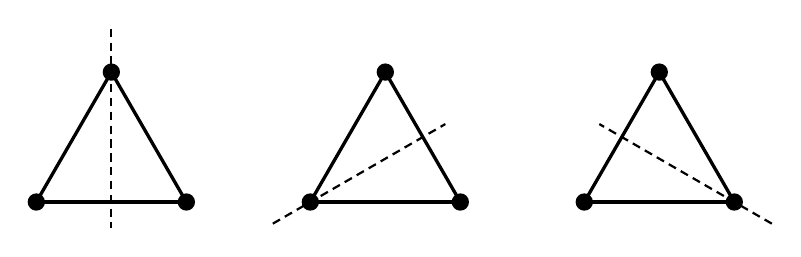
\begin{tikzpicture}[scale=1.1]
            % first triangle
            \fill[black] (90:1) circle (0.1);
            \fill[black] (210:1) circle (0.1);
            \fill[black] (330:1) circle (0.1);
            \draw[very thick] (90:1) -- (210:1);
            \draw[very thick] (210:1) -- (330:1);
            \draw[very thick] (330:1) -- (90:1);
            \draw[thick, densely dashed] (90:1.5) -- (270:0.8);
            % second triangle
            \fill[black] ([xshift=9em]90:1) circle (0.1);
            \fill[black] ([xshift=9em]210:1) circle (0.1);
            \fill[black] ([xshift=9em]330:1) circle (0.1);
            \draw[very thick] ([xshift=9em]90:1) -- ([xshift=9em]210:1);
            \draw[very thick] ([xshift=9em]210:1) -- ([xshift=9em]330:1);
            \draw[very thick] ([xshift=9em]330:1) -- ([xshift=9em]90:1);
            \draw[thick, densely dashed] ([xshift=9em]210:1.5) -- ([xshift=9em]30:0.8);
          % third triangle
            \fill[black] ([xshift=18em]90:1) circle (0.1);
            \fill[black] ([xshift=18em]210:1) circle (0.1);
            \fill[black] ([xshift=18em]330:1) circle (0.1);
            \draw[very thick] ([xshift=18em]90:1) -- ([xshift=18em]210:1);
            \draw[very thick] ([xshift=18em]210:1) -- ([xshift=18em]330:1);
            \draw[very thick] ([xshift=18em]330:1) -- ([xshift=18em]90:1);
            \draw[thick, densely dashed] ([xshift=18em]330:1.5) -- ([xshift=18em]150:0.8);
          \end{tikzpicture}
        \end{center}

      \item
        Ist $n$ gerade, so gibt es zwei Arten von Spiegelungen:
        \begin{itemize}
          \item
            Es gibt $n/2$ Spiegelungen, deren Spiegelungsachse jeweils durch den Mittelpunkt einer Kante sowie den Mittelpunkt der gegenüberliegenden Kante gehen.
            \begin{center}
              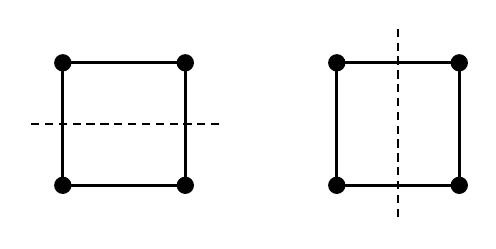
\begin{tikzpicture}[scale=1.1]
                % first square
                \fill[black] (45:1) circle (0.1);
                \fill[black] (135:1) circle (0.1);
                \fill[black] (225:1) circle (0.1);
                \fill[black] (315:1) circle (0.1);
                \draw[very thick] (45:1) -- (135:1);
                \draw[very thick] (135:1) -- (225:1);
                \draw[very thick] (225:1) -- (315:1);
                \draw[very thick] (315:1) -- (45:1);
                \draw[thick, densely dashed] (0:1.1) -- (180:1.1);
                % second square
                \fill[black] ([xshift=9em]45:1) circle (0.1);
                \fill[black] ([xshift=9em]135:1) circle (0.1);
                \fill[black] ([xshift=9em]225:1) circle (0.1);
                \fill[black] ([xshift=9em]315:1) circle (0.1);
                \draw[very thick] ([xshift=9em]45:1) -- ([xshift=9em]135:1);
                \draw[very thick] ([xshift=9em]135:1) -- ([xshift=9em]225:1);
                \draw[very thick] ([xshift=9em]225:1) -- ([xshift=9em]315:1);
                \draw[very thick] ([xshift=9em]315:1) -- ([xshift=9em]45:1);
                \draw[thick, densely dashed] ([xshift=9em]90:1.1) -- ([xshift=9em]270:1.1);
              \end{tikzpicture}
            \end{center}
          \item
            Es gibt $n/2$ Spiegelungen, deren Spiegelungsachse jeweils durch einen Eckpunkt sowie den gegenüberliegenden Eckpunkt gehen.
            \begin{center}
              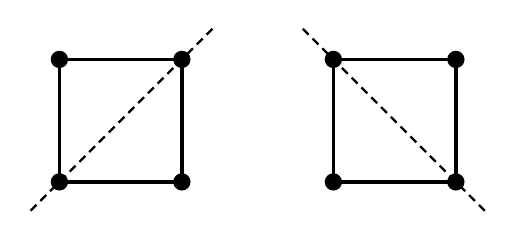
\begin{tikzpicture}[scale=1.1]
                % first square
                \fill[black] (45:1) circle (0.1);
                \fill[black] (135:1) circle (0.1);
                \fill[black] (225:1) circle (0.1);
                \fill[black] (315:1) circle (0.1);
                \draw[very thick] (45:1) -- (135:1);
                \draw[very thick] (135:1) -- (225:1);
                \draw[very thick] (225:1) -- (315:1);
                \draw[very thick] (315:1) -- (45:1);
                \draw[thick, densely dashed] (45:1.5) -- (225:1.5);
                % second square
                \fill[black] ([xshift=9em]45:1) circle (0.1);
                \fill[black] ([xshift=9em]135:1) circle (0.1);
                \fill[black] ([xshift=9em]225:1) circle (0.1);
                \fill[black] ([xshift=9em]315:1) circle (0.1);
                \draw[very thick] ([xshift=9em]45:1) -- ([xshift=9em]135:1);
                \draw[very thick] ([xshift=9em]135:1) -- ([xshift=9em]225:1);
                \draw[very thick] ([xshift=9em]225:1) -- ([xshift=9em]315:1);
                \draw[very thick] ([xshift=9em]315:1) -- ([xshift=9em]45:1);
                \draw[thick, densely dashed] ([xshift=9em]135:1.5) -- ([xshift=9em]315:1.5);
              \end{tikzpicture}
            \end{center}
        \end{itemize}
    \end{itemize}
    Damit ergeben sich insgesamt $2n$ Isometrien.
    
  \item
    Es sei $x$ einer der Eckpunkte und $x'$ ein zu $x$ benachbarter Eckpunkt.
    Dann ist jede Isometrie des $n$-Ecks durch die Wirkung auf den benachbarten Eckpunkten $x$ und $x'$ bereits eindeutig bestimmt.
    
    Der Eckpunkt $x$ kann auf jeden Eckpunkte abgebildet werden, wofür es $n$ Möglichkeiten gibt.
    Wird der Eckpunkt $x$ auf einen Eckpunkt $y$ abgebildet, so kann $x'$ auf jeden der beiden zu $y$ benachbarten Eckpunkte abgebildet werden.
    
    Somit ergeben sich $2n$ Isometrien
\end{itemize}

Um zu zeigen, dass $D_n$ nicht abelsch ist, nummerieren wir die Eckpunkte des $n$-Ecks mit den Elementent von $\Integer/n$, so dass der Eckpunkt $\class{k}$ mit den Eckpunkten $\class{k-1}$ und $\class{k+1}$ benachbart sind.
\begin{center}
  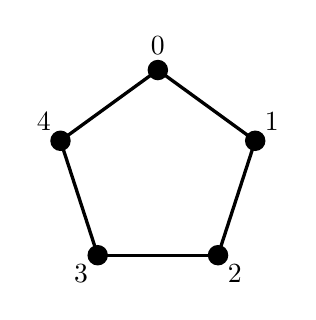
\begin{tikzpicture}[scale=1.3]
    \fill[black] (90:1) circle (0.1) node[above=2]{$\class{0}$};
    \fill[black] (162:1) circle (0.1) node[anchor=south east]{$\class{4}$};
    \fill[black] (234:1) circle (0.1) node[anchor=north east]{$\class{3}$};
    \fill[black] (306:1) circle (0.1) node[anchor=north west]{$\class{2}$};
    \fill[black] (18:1) circle (0.1) node[anchor=south west]{$\class{1}$};
    \draw[very thick] (90:1) -- (162:1);
    \draw[very thick] (162:1) -- (234:1);
    \draw[very thick] (234:1) -- (306:1);
    \draw[very thick] (306:1) -- (18:1);
    \draw[very thick] (18:1) -- (90:1);
  \end{tikzpicture}
\end{center}


Die Rotation um $360^\circ/n$ ist dann durch
\[
          r
  \colon  \Integer/n
  \to     \Integer/n,
  \quad   \class{k}
  \mapsto \class{k+1}
\]
gegeben.
Die Spiegelung, deren Achse durch den Eckpunkt $\class{0}$ geht, ist dann durch
\[
          r
  \colon  \Integer/n
  \to     \Integer/n,
  \quad   \class{k}
  \mapsto \class{-k}
\]
gegeben.
Es gilt
\begin{gather*}
    (r \circ s)(\class{0})
  = r(s(\class{0}))
  = r(\class{0})
  = \class{1}
\shortintertext{aber}
    (s \circ r)(\class{0})
  = s(r(\class{0}))
  = s(\class{1})
  = \class{-1},
\end{gather*}
wobei $\class{1} \neq \class{-1}$ da $n \geq 3$.

\begin{center}
  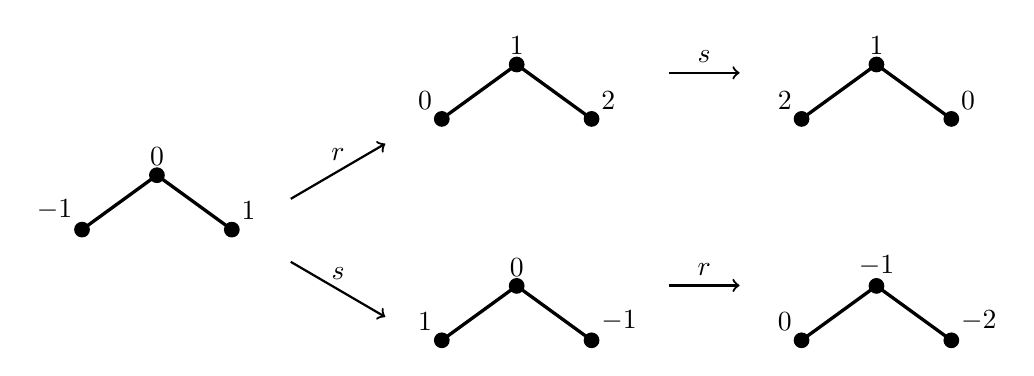
\begin{tikzpicture}[scale=1]
    % basic one
    \fill[black] (90:1) circle (0.1) node[anchor=south]{$\class{0}$};
    \fill[black] (162:1) circle (0.1) node[anchor=south east]{$\class{-1}$};
    \fill[black] (18:1) circle (0.1) node[anchor=south west]{$\class{1}$};
    \draw[very thick] (90:1) -- (162:1);
    \draw[very thick] (18:1) -- (90:1);
    % rotated
    \fill[black] ([xshift=13em, yshift=4em]90:1) circle (0.1) node[anchor=south]{$\class{1}$};
    \fill[black] ([xshift=13em, yshift=4em]162:1) circle (0.1) node[anchor=south east]{$\class{0}$};
    \fill[black] ([xshift=13em, yshift=4em]18:1) circle (0.1) node[anchor=south west]{$\class{2}$};
    \draw[very thick] ([xshift=13em, yshift=4em]90:1) -- ([xshift=13em, yshift=4em]162:1);
    \draw[very thick] ([xshift=13em, yshift=4em]18:1) -- ([xshift=13em, yshift=4em]90:1);
    % rotated then reflected
    \fill[black] ([xshift=26em, yshift=4em]90:1) circle (0.1) node[anchor=south]{$\class{1}$};
    \fill[black] ([xshift=26em, yshift=4em]162:1) circle (0.1) node[anchor=south east]{$\class{2}$};
    \fill[black] ([xshift=26em, yshift=4em]18:1) circle (0.1) node[anchor=south west]{$\class{0}$};
    \draw[very thick] ([xshift=26em, yshift=4em]90:1) -- ([xshift=26em, yshift=4em]162:1);
    \draw[very thick] ([xshift=26em, yshift=4em]18:1) -- ([xshift=26em, yshift=4em]90:1);
    % reflected
    \fill[black] ([xshift=13em, yshift=-4em]90:1) circle (0.1) node[anchor=south]{$\class{0}$};
    \fill[black] ([xshift=13em, yshift=-4em]162:1) circle (0.1) node[anchor=south east]{$\class{1}$};
    \fill[black] ([xshift=13em, yshift=-4em]18:1) circle (0.1) node[anchor=south west]{$\class{-1}$};
    \draw[very thick] ([xshift=13em, yshift=-4em]90:1) -- ([xshift=13em, yshift=-4em]162:1);
    \draw[very thick] ([xshift=13em, yshift=-4em]18:1) -- ([xshift=13em, yshift=-4em]90:1);
    % reflected then rotated
    \fill[black] ([xshift=26em, yshift=-4em]90:1) circle (0.1) node[anchor=south]{$\class{-1}$};
    \fill[black] ([xshift=26em, yshift=-4em]162:1) circle (0.1) node[anchor=south east]{$\class{0}$};
    \fill[black] ([xshift=26em, yshift=-4em]18:1) circle (0.1) node[anchor=south west]{$\class{-2}$};
    \draw[very thick] ([xshift=26em, yshift=-4em]90:1) -- ([xshift=26em, yshift=-4em]162:1);
    \draw[very thick] ([xshift=26em, yshift=-4em]18:1) -- ([xshift=26em, yshift=-4em]90:1);
    % arrows
    \draw[thick, ->] (1.7, 0.7) -- node[above]{$r$} (2.9,  1.4);
    \draw[thick, ->] (1.7, -0.1) -- node[above]{$s$} (2.9, -0.8);
    \draw[thick, ->] (6.5, 2.3) -- node[above]{$s$} (7.4, 2.3);
    \draw[thick, ->] (6.5, -0.4) -- node[above]{$r$} (7.4, -0.4);
  \end{tikzpicture}
\end{center}






\subsection{}

Das regelmäßige $n$-Eck lässt sich in die Ebene $\Real^2$ einbetten, so dass der Nullpunkt $(0,0)$ der Schwerpunkt des $n$-Ecks ist, und einer der Eckpunkte der $n$-Ecks auf der $x$-Achse liegt.
\begin{center}
  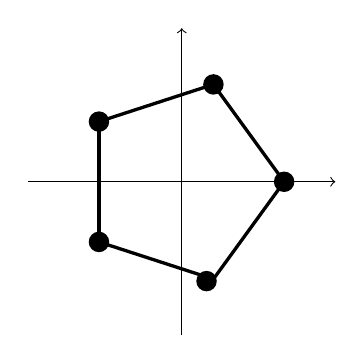
\begin{tikzpicture}[scale=1.3]
    \draw[->] (-1.5,0) -- (1.5,0);
    \draw[->] (0,-1.5) -- (0,1.5);
    \fill[black] (0:1) circle (0.1);
    \fill[black] (72:1) circle (0.1);
    \fill[black] (144:1) circle (0.1);
    \fill[black] (216:1) circle (0.1);
    \fill[black] (284:1) circle (0.1);
    \draw[very thick] (0:1)   -- (72:1);
    \draw[very thick] (72:1)  -- (144:1);
    \draw[very thick] (144:1) -- (216:1);
    \draw[very thick] (216:1) -- (288:1);
    \draw[very thick] (288:1) -- (0:1);
  \end{tikzpicture}
\end{center}
Dann lassen sich die Elemente von $D_n$ als Rotationen und Spiegelungen der Ebene auffassen, und somit als Rotations- und Spiegelungsmatrizen.
Für $\alpha \in \Real$ ist die Rotation um den Winkel $\alpha$ durch die Matrix
\[
            R_\alpha
  \coloneqq \begin{pmatrix*}[r]
              \cos \alpha & -\sin \alpha  \\
              \sin \alpha &  \cos \alpha
            \end{pmatrix*}
\]
gegeben, und die Spiegelung an der Gerade mit Winkel $\alpha$ (zur $x$-Achse) ist durch die Matrix
\[
            S_\alpha
  \coloneqq \begin{pmatrix*}[r]
              \cos 2\alpha  &  \sin 2\alpha \\
              \sin 2\alpha  & -\cos 2\alpha
            \end{pmatrix*}
\]
gegeben.
Die Gruppe $D_n$ ist dann durch die Matrizen
\[
            \hat{D}_n
  \coloneqq \{
              R_{k 2\pi/n}
            \suchthat
              k = 0, \dotsc, n-1
            \}
            \cup
            \{
              S_{k \pi/n}
            \suchthat
              k = 0, \dotsc, n-1
            \}
\]
gegeben.
Es ist $\hat{D}_n \subgroup \orthogonal{2}$ eine Untergruppe, weshalb wir den surjektiven Gruppenhomomorphismus $\restrict{\det}{\orthogonal{2}} \colon \orthogonal{2} \to \{1, -1\}$ zu einem Gruppenhomomorphismus $\restrict{\det}{\hat{D}_n} \colon \hat{D}_n \to \{1,-1\}$ einschränken können.
Es gilt $\det R_\alpha = 1$ und $\det S_\alpha = -1$ für alle $\alpha \in \Real$, weshalb auch $\restrict{\det}{\hat{D}_n}$ noch surjektiv ist.
Damit erhalten wir einen surjektiven Gruppenhomomorphismus
\[
          \hat{g}
  \colon  D_n
  \to     \{1, -1\},
  \quad   x
  \mapsto \begin{cases}
            \phantom{-}1  & \text{falls $x$ eine Rotation ist}, \\
                      -1  & \text{falls $x$ eine Spiegelung ist}.
          \end{cases}
\]
Da $\{1, -1\} \cong \Integer/2$ gilt, lässt sich $\hat{g}$ auch als ein Gruppenhomomorphismus
\[
          g
  \colon  D_n
  \to     \Integer/2,
  \quad   x
  \mapsto \begin{cases}
            \class{0} & \text{falls $x$ eine Rotation ist}, \\
            \class{1} & \text{falls $x$ eine Spiegelung ist},
          \end{cases}
\]
auffassen.





\subsection{}

Der Kern von $g$ besteht genau aus der Untergruppe der Rotationen.

Jedes Element $x \in D_n$ liefert einen Gruppenhomomorphismus
\[
          \tilde{s}
  \colon  \Integer
  \to     D_n\,,
  \quad   n
  \mapsto x^n\,.
\]
Ist $x$ eine Spiegelung, so gilt $x \neq 1$ aber $x^2 = 1$, und somit $\ker \tilde{s} = 2\Integer$.
Somit induziert $\tilde{s}$ einen wohldefinierten Gruppenhomomorphismus
\[
          s
  \colon  \Integer/2
  \to     D_n\,,
  \quad   \class{n}
  \mapsto x^n\,.
\]
Dann gilt
\[
    (g \circ s)(\class{1})
  = g(s(\class{1}))
  = g(x^1)
  = g(x)
  = \class{1}\,,
\]
sowie $(g \circ s)(\class{0}) = \class{0}$ da $g \circ s$ ein Gruppenhomomorphismus ist.
Somit gilt $g \circ s = \id_{\Integer/2}$.





\subsection*{Bemerkungen}

\begin{remark}
  Manche Autoren schreiben $D_{2n}$ statt $D_n$, d.h.\ $D_{2n}$ ist die Diedergruppe von Ordnung $2n$.
\end{remark}


\begin{remark}
  Ist $r \in D_n$ eine Rotation um den Winkel $2\pi/n$ und $s \in D_n$ eine Spiegelung, so gilt
  \begin{itemize}
    \item
      $\ord{r} = n$,
    \item
      $\ord{s} = 2$,
    \item
      $s r = r^{-1} s$.
  \end{itemize}
  Durch diese Bedingungen sind die Elemente und die Gruppenstruktur von $D_n$ bereits eindeutig bestimmt:
  \begin{itemize}
    \item
      Es gilt $\generated{r} = \{1, r, \dotsc, r^{n-1}\}$ mit $\card{ \generated{r} } = n$.
      Für $\generated{r} s = \{s, rs, \dotsc, r^{n-1} s\}$ gilt dann ebenfalls $\card{ \generated{r} s } = n$, da die Abbildung $D_n \to D_n$, $x \mapsto xs$ bijektiv ist.
    \item
      Es gilt $s \notin \generated{r}$, da $s$ keine Rotation ist.
      Deshalb sind $\generated{r}$ und $\generated{r} s$ disjunkt.
    \item
      Da $\card{D_n} = 2n = n + n = \card{\generated{r}} + \card{\generated{r} s}$ gilt, ist $D_n$ bereits die disjunkte Vereinigung von $\generated{r}$ und $\generated{r} s$.
      Es lässt sich also jedes Element $x \in D_n$ als $x = r^i s^j$ mit eindeutigen $0 \leq i \leq n-1$ und $0 \leq j \leq 1$ darstellen.
  \end{itemize}
  Das zeigt, dass die Elemente von $D_n$ eindeutig bestimmt sind.
  \begin{itemize}[resume]
    \item
      Aus $s r = r^{-1} s$ folgt, dass $s r s^{-1} = r$.
      Da die Abbildung $c \colon G \to G$, $x \mapsto s x s^{-1}$ ein Gruppenhomomorphismus ist, folgt ferner, dass bereits $s r^i s^{-1} = r^{-i}$ für alle $i \in \Integer$ gilt.
      Für alle $i \in \Integer$ und $j \in \Integer$ gilt deshalb $s^j r^i = r^{(-1)^j i} s^j$ (da $s^2 = 1$ gilt, genügt es, dass dies für $j = 0, 1$ gilt).
    \item
      Für alle $i, j, k , l \in \Integer$ gilt somit
      \[
          r^i s^j r^k s^l
        = r^i r^{(-1)^j k} s^j s^l
        = r^{i + (-1)^j } s^{j + l}
        = r^{(i + (-1)^j) \bmod 2} s^{(j + l) \bmod 2}
      \]
  \end{itemize}
  Also ist auch die Gruppenstruktur auf $D_n$ bereits bestimmt.
\end{remark}

Inbesondere ließe sich die Diedergruppe $D_n$ auch auf rein algebraische Weise als die Menge $(\Integer/n) \times (\Integer/2)$ zusammen mit der Verknüpfung
\begin{equation}
  \label{equation: algebraic construction of the dihedral group}
            (\class{i}, \class{j}) \cdot (\class{k}, \class{l})
  \coloneqq (\class{i} + (-1)^j \class{k}, \class{j} + \class{l})
\end{equation}
definieren.

\begin{remark}
  Auf diese Weise lassen sich auch die Gruppen $D_1$ und $D_2$ definieren:
  \begin{itemize}
    \item
      Die Gruppe $D_1$ lässt sich als die Menge $(\Integer/1) \times (\Integer/2)$ zusammen mit der Verknüpfung~\eqref{equation: algebraic construction of the dihedral group} definieren.
      Dann ist die Bijektion $(\Integer/1) \times (\Integer/2) \to \Integer/2$, $(x,y) \mapsto y$ ein Gruppenhomomorphismus, und somit $D_1 \cong \Integer/2$.
    \item
      Die Gruppe $D_1$ lässt sich als die Menge $(\Integer/2) \times (\Integer/2)$ zusammen mit der Verknüpfung~\eqref{equation: algebraic construction of the dihedral group} definieren.
      Für die Gruppe $P \coloneqq (\Integer/2) \times (\Integer/2)$ mit der \enquote{üblichen} Pro\-dukt-Gruppen\-struk\-tur ist dann die Abbildung
      \[
                P
        \to     D_2,
        \quad   (x, y)
        \mapsto (x+y,y)
      \]
      ein Gruppenhomomorphismus, und somit $D_2 \cong \Integer/2 \times \Integer/2$ als Gruppen.
  \end{itemize}
  
  Ähnlich wie die Diedergruppen $D_n$ mit $n \geq 3$ lassen sich auch die Diedergruppen $D_1$ und $D_2$ geometrisch definieren:
  Das regelmäßige $1$-Eck und $2$-Eck lassen sich wie folgt in $\Real^2$ einbetten:
  \begin{center}
    \begin{tikzpicture}
      \draw[very thin, ->] (-2,0) -- (2,0) node[anchor = west, black] {$x$};
      \draw[very thin, ->] (0,-2) -- (0,2) node[anchor = south, black] {$y$};
      \fill (1,0) circle (0.1);
    \end{tikzpicture}
    \hspace{2em}
    \begin{tikzpicture}
      \draw[very thin, ->] (-2,0) -- (2,0) node[anchor = west, black] {$x$};;
      \draw[very thin, ->] (0,-2) -- (0,2) node[anchor = south, black] {$y$};
      \fill (-1,0) circle (0.1);
      \fill (1,0) circle (0.1);
      \draw[very thick] (-1,0) -- (1,0);
    \end{tikzpicture}
  \end{center}
  Die Diedergruppe $D_n$ für $n = 1, 2$ besteht dann aus all jeden Isometrien der umgebenen Ebene $\Real^2$, welche diese eingebettete Version des $n$-Ecks unverändert lassen:
  \begin{itemize}
    \item
      Die Diedergruppe $D_1$ besteht also aus all jenen Isometrien der Ebene, welche den Punkt $(1,0)$ unverändert lassen.
      Hierfür kommen nur die Identität und die Spiegelung an der $x$-Achse in Frage.
      Somit gilt $D_1 \cong \Integer/2$.
    \item
      Die Diedergruppe $D_2$ besteht aus all jenen Isometrien der Ebene, welche das eingezeichnete Interval $[-1, 1] \times \{0\}$ unverändert lassen.
      Dies sind die Identität, die Spiegelungen an den beiden Achsen, sowie die Komposition dieser beiden Spiegelungen (welche die Spiegelung am Koordinatenursprung ist).
      Da die Spiegelungen an den Achsen miteinander kommutieren, ergibt sich, dass $D_2 \cong \Integer/2 \times \Integer/2$.
  \end{itemize}
\end{remark}





